% !TeX root = ../master.tex

\lecture{10}{2026-09-29}{Makromekanik for Laminater, Pt. II}

\subsection{Koblinger i CLT}
Vi betragter ABD-matricerne for CLT ovenfor.
Heri er hhv $A_{16}$ og $A_{26}$ shear-extension kobling -- Dette er analogt til shear-extension koblingen fra \Mref{sec:kobling1}.
Hele $\Mat{B}$ er beinding-extension kobling, hvilket ikke er et fænomen for enkelte lamina.
Slutteligt er $D_{16}$ og $D_{26}$ er bend-twist kobling \citepage{jones2021mechanicscompositematerials}{200}.

\begin{figure} [ht]
  \centering
  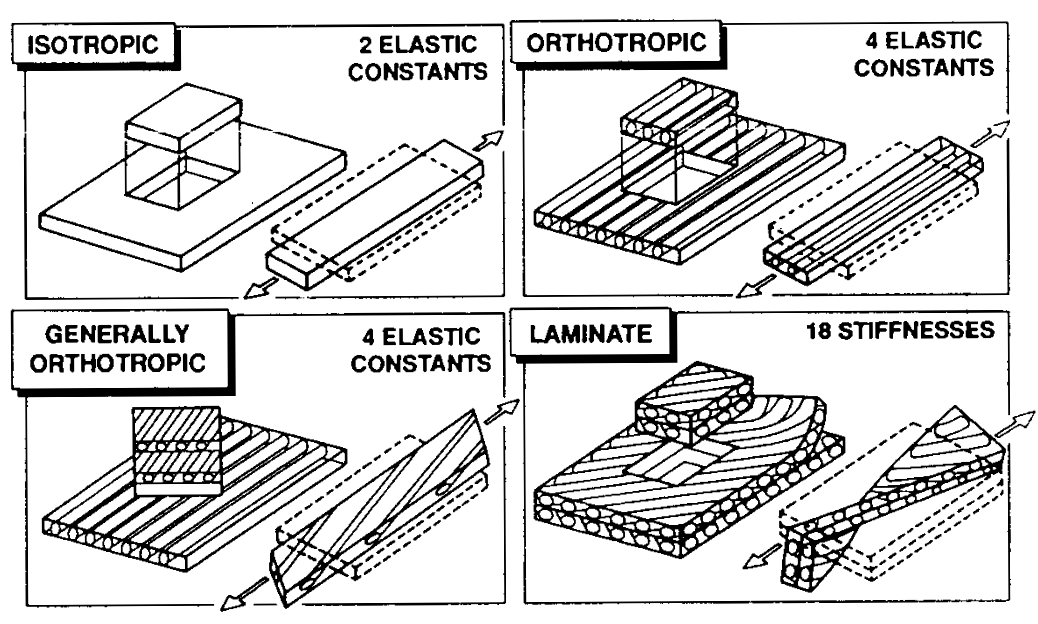
\includegraphics[width=0.7\linewidth]{./figures/elasconst.png}
  \caption{Antal elastiske Konstanter for isotropiske, specielt ortotropiske, generelt ortotropiske og generelle laminater. Reproduceret fra \citepage{jones2021mechanicscompositematerials}{Fig 4--13}.}
  \label{fig:elasconst}
\end{figure}

På \Mref{fig:elasconst} er vist generelle former efter aksial belastning samt antal uafhængige elastiske konstanter for isotrope, specielt ortotrope (load i fiberretning), generelt ortotrope, og generelle laminater.
Bemærk at shear-extension kobling ikke sker for specielt ortotrope laminater men opstår for generelt ortotrope laminater.
Bemærk i øvrigt også, at et laminat har maksimalt 18 stivheder (seks i hver a $\Mat{A}, \Mat{B}, \Mat{D}$).
Der er maksimalt 4 elastiske konstanter i et laminat per lag, men hvis laminatet har samme materiale i alle lag, så har det kun 4 elastiske konstanter.

\subsubsection{Laminat-terminologi og -koblinger}
\paragraph{Symmetrisk Laminat}
Et symmetrisk laminat er symmetrisk både ift. geometri og materiale-egenskaber på begge sider af laminatets midterlinje.
Her er der ingen bending-extension, $\Mat{B} = 0$.
Et eksempel på et layup her er $[-45,45,45,-45] = [-45,45]_s$.

\paragraph{Anti-symmetrisk Laminat}
Geometrisk symmetri omkring midterlinjen, men reverserede materiale-egenskaber.
Her er der ingen bending-twist og shear-extension, altså $A_{16} = A_{26} = D_{16} = D_{26} = 0$.
Et eksempel på et layup her et $[-45,45,-45,45]=[-45,45]_2$.

\paragraph{Asymmetrisk Laminat}
Ingen symmetri overhovedet.
Her er et eksempel på et layup $[-5,40,-90,-55]$.

\paragraph{Balanceret Laminat}
Alle lamina har samme tykkelse og materiale-egenskaber.
Derudover er der for hver $-\theta$-ply et tilsvarende $\theta$-ply.
Her forekommer ikke shear-extension, $A_{16} = A_{26} = 0$.
Et eksempel på et layup her er $[-5,5,90,-90]=[\mp 5, \pm 90]$.

\paragraph{Regulært Laminat}
Alle lamina har samme tykkelse.
Et eksempel på et layup kunne være $[-60,60,-60,60]=[\mp60]_2$.

\paragraph{Kvasi-isotropisk Laminat}
Laminat har ens extensional stivhed i planet.
Dette opnås ved jævn fordeling af fiber-vinkler.
Et eksempel på et layup er $[-45,0,45,90]$

\paragraph{Kombinationer}
Dette er kombinationer af de tidligere, hvor ingen af deres individuelle definitioner brydes.
Her er inden bending-twist og shear-extension.
Bending-extension går mod 0 for højere antal lag.

Et eksempel på et regulært anti-symmetrisk kombinations layup er $[-60,60,-60,60]=[\mp60]_2$.
Et balanceret assymetrisk kombinations-layup kunne være $[-5,5,90,-90]=[\mp5, \pm90]$.

\paragraph{Øvrig Laminatterminologi}
Arbejder man med forskellige materialer i sit layup, eksempelvis $CF$ og $GF$ kan layuppet skrives som $[CF@-60,GF@30,GF@-60,CF@0]$.
Har man forskellige materialetykkelser kan det angives som $[-5@3t,5@t,65@4t,-65@t]$.

\paragraph{Øvrige Specialtilfælde af ABD-Matricerne for CLT}
For enkeltlagslaminater er der ingen bending-extension, $\Mat{B} = 0$.
For symmetriske balancerede lamina er der ingen bending-extension, $\Mat{B} = 0$ og shear-extension $A_{16} = A_{26} = 0$.
Cross-ply laminater $[0,90,\ldots ]$ er ortotropiske, så $A_{16} = A_{26} = B_{16} = B_{26} = D_{16} = D_{26} = 0$.
Kvasi-isotropiske laminater har isotopi i planet, altså $A_{11} = A_{22}$, $A_{12} = \nu A_{11}$, $A_{66} = (1-\nu) / 2 A_{11}$, og $A_{16} = A_{26} = 0$.
